\documentclass[aspectratio=169]{beamer}
\usetheme{metropolis}

\usepackage{booktabs}
\usepackage{multirow}
\usepackage{amsmath}
\usepackage{graphicx}
\usepackage{hyperref}
\usepackage[normalem]{ulem} % for \sout (strikethrough)
\usetikzlibrary{positioning, fit, arrows.meta, calc, decorations.pathreplacing}

\graphicspath{{../docs/}{../}{./figures/}}

\definecolor{insared}{HTML}{CC2B1E}
\definecolor{vcolor}{HTML}{2E86AB}
\definecolor{mcolor}{HTML}{E8871E}
\definecolor{ccolor}{HTML}{7FB069}
\setbeamercolor{progress bar}{fg=insared}
\setbeamertemplate{frame footer}{}
\metroset{block=fill}
% Reduce frame title spacing to prevent overflow
\addtobeamertemplate{frametitle}{}{\vspace*{-0.3em}}

\title{DeepDash}
\subtitle{World Models for Geometry Dash}
\author{Florent Tariolle \& Maël Planchot}
\institute{INSA Rouen Normandie \\ Representation Learning}
\date{}

% ============================================================
\begin{document}

% --- Title ---
{%
\setbeamertemplate{headline}{}
\begin{frame}[noframenumbering,plain]
  \begin{tikzpicture}[remember picture,overlay]
    \node[anchor=north east,yshift=-0.4cm,xshift=-0.4cm] at (current page.north east) {
\includegraphics[height=0.9cm]{school_logo.png}};
  \end{tikzpicture}
  \titlepage
\end{frame}
}

% ==========================================================
\section{Motivation}
% ==========================================================

\begin{frame}{Why World Models?}
  \begin{itemize}
    \item Model-free RL (DQN, PPO) requires \textbf{millions of environment interactions}
    \item World Models (Ha \& Schmidhuber, 2018): learn a \textbf{compressed model of the environment}, then train a controller entirely \textbf{in imagination}
    \item \textbf{Geometry Dash}: deterministic physics, binary action (jump/idle), precision timing. Ideal testbed for latent dynamics learning
  \end{itemize}

  \vspace{0.5em}
  \textbf{Goal}: master Geometry Dash levels by training a controller entirely \emph{in imagination}
\end{frame}

% ==========================================================
\section{Architecture Overview}
% ==========================================================

\begin{frame}{V $\to$ M $\to$ C: High-Level Pipeline}
  \vspace{1em}
  \begin{center}
  \resizebox{\textwidth}{!}{%
  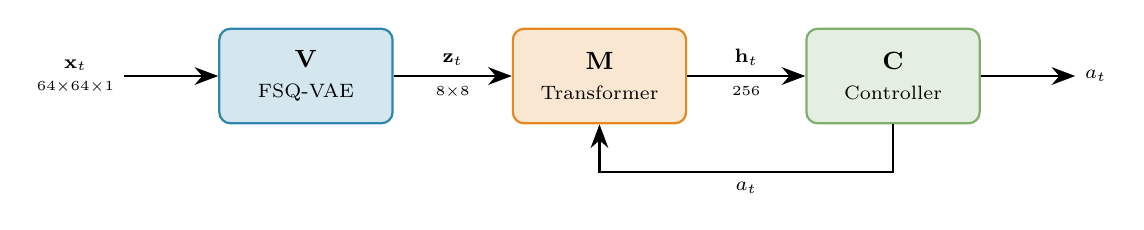
\begin{tikzpicture}[
    block/.style={rectangle, draw, rounded corners, minimum height=1.2cm, minimum width=2.2cm, align=center, font=\small, line width=0.8pt},
    arr/.style={-{Stealth[length=3mm]}, thick},
    lbl/.style={font=\scriptsize, align=center},
  ]
    \node[block, fill=vcolor!20, draw=vcolor] (V) {\textbf{V}\\\scriptsize FSQ-VAE};
    \node[block, fill=mcolor!20, draw=mcolor, right=1.5cm of V] (M) {\textbf{M}\\\scriptsize Transformer};
    \node[block, fill=ccolor!20, draw=ccolor, right=1.5cm of M] (C) {\textbf{C}\\\scriptsize Controller};

    \node[left=1.2cm of V, lbl] (input) {$\mathbf{x}_t$\\{\tiny 64$\times$64$\times$1}};
    \node[right=1.2cm of C, lbl] (output) {$a_t$};

    \draw[arr] (input) -- (V);
    \draw[arr] (V) -- node[above, lbl] {$\mathbf{z}_t$} node[below, lbl] {\tiny 8$\times$8} (M);
    \draw[arr] (M) -- node[above, lbl] {$\mathbf{h}_t$} node[below, lbl] {\tiny 256} (C);
    \draw[arr] (C) -- (output);

    \draw[arr] (C.south) -- ++(0,-0.6) -| node[below, lbl, pos=0.25] {$a_t$} (M.south);
  \end{tikzpicture}%
  }
  \end{center}

  \vspace{0.5em}
  \begin{center}
    \small
    $\mathbf{x}_t \in \mathbb{R}^{64 \times 64}$: grayscale Sobel frame \quad\quad
    $\mathbf{z}_t \in \{0,\ldots,999\}^{64}$: discrete tokens \\[0.3em]
    $\mathbf{h}_t \in \mathbb{R}^{256}$: hidden state \quad\quad
    $a_t \in \{0, 1\}$: jump/idle
  \end{center}
\end{frame}

% ==========================================================
\section{Data Collection}
% ==========================================================

\begin{frame}{Data Collection}
  \begin{center}
    \begin{tabular}{cccc}
      
\includegraphics[width=0.2\textwidth]{preprocessing_1_original.png} &
      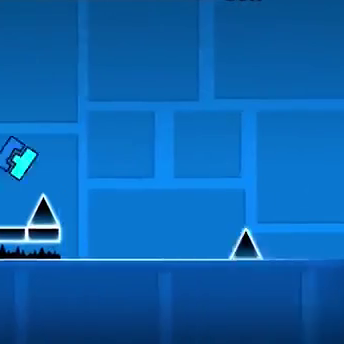
\includegraphics[width=0.2\textwidth]{preprocessing_2_cropped.png} &
      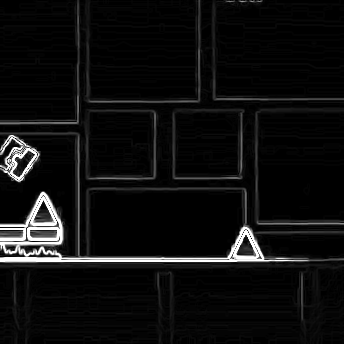
\includegraphics[width=0.2\textwidth]{preprocessing_3_sobel.png} &
      
\includegraphics[width=0.2\textwidth]{preprocessing_4_final.png} \\
      {\scriptsize Raw 1080p} & {\scriptsize Square crop} & {\scriptsize Sobel edges} & {\scriptsize 64$\times$64}
    \end{tabular}
  \end{center}

  \begin{itemize}
    \item Live gameplay at \textbf{30 FPS}, death detection via process memory reading
    \item Frames + actions recorded simultaneously, saved as \texttt{.npy} per episode
    \item \textbf{Death episodes}: $\sim$3,600 episodes, $\sim$180K frames (intentional deaths at obstacles)
    \item \textbf{Expert episodes}: $\sim$36 clean runs, $\sim$33K frames (no deaths, for BC + rebalancing world model)
  \end{itemize}
\end{frame}

% ==========================================================
\section{Phase 1: V (FSQ-VAE)}
% ==========================================================

\begin{frame}{Vision Model: $\beta$-VAE $\to$ VQ-VAE $\to$ FSQ-VAE}
  \begin{itemize}
    \item \textbf{$\beta$-VAE}: Gaussian posterior $\Rightarrow$ always blurry. No spatial structure.
    \item \textbf{VQ-VAE}: discrete, spatially localized tokens $\Rightarrow$ sharp. But codebook collapse, commitment cost tuning.
    \item \textbf{FSQ-VAE} (Mentzer et al., 2023): round to $L$ fixed levels. No codebook, no auxiliary losses, 100\% utilization by construction.
  \end{itemize}

  \vspace{0.3em}
  \begin{center}
    Levels $[8,5,5,5]$ $\Rightarrow$ 1000 codes, $8\times8$ grid $=$ \textbf{64 tokens/frame}
  \end{center}
  % TODO: add before/after reconstruction comparison
\end{frame}

\begin{frame}{FSQ-VAE: Architecture}
  \vspace{0.5em}
  \begin{center}
  \resizebox{0.9\textwidth}{!}{%
  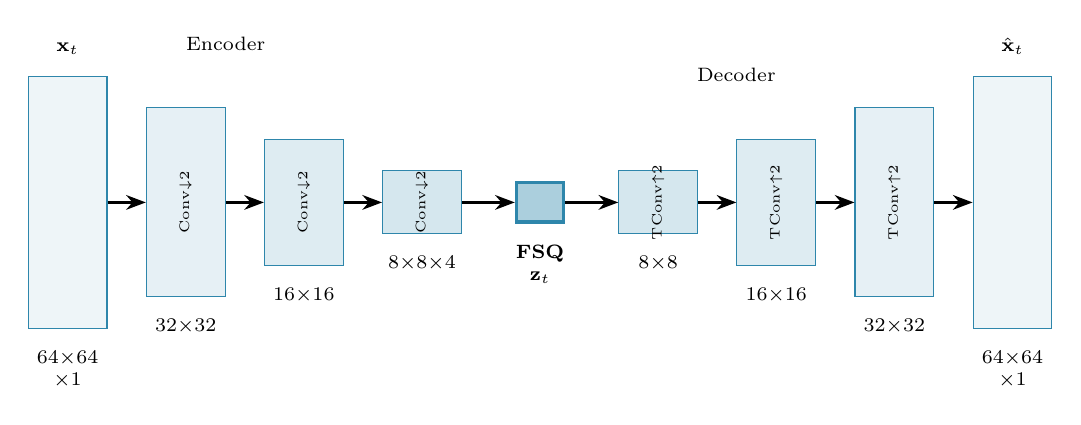
\begin{tikzpicture}[
    arr/.style={-{Stealth[length=2.5mm]}, thick},
    lbl/.style={font=\scriptsize, align=center},
  ]
    % Encoder pyramid (height = spatial size, width constant)
    \node[rectangle, draw=vcolor, fill=vcolor!8, minimum width=1cm, minimum height=3.2cm] (e0) at (0,0) {};
    \node[rectangle, draw=vcolor, fill=vcolor!12, minimum width=1cm, minimum height=2.4cm] (e1) at (1.5,0) {};
    \node[rectangle, draw=vcolor, fill=vcolor!16, minimum width=1cm, minimum height=1.6cm] (e2) at (3,0) {};
    \node[rectangle, draw=vcolor, fill=vcolor!20, minimum width=1cm, minimum height=0.8cm] (e3) at (4.5,0) {};

    % FSQ bottleneck
    \node[rectangle, draw=vcolor, fill=vcolor!40, minimum width=0.6cm, minimum height=0.5cm, line width=1.2pt] (fsq) at (6,0) {};

    % Decoder pyramid
    \node[rectangle, draw=vcolor, fill=vcolor!20, minimum width=1cm, minimum height=0.8cm] (d1) at (7.5,0) {};
    \node[rectangle, draw=vcolor, fill=vcolor!16, minimum width=1cm, minimum height=1.6cm] (d2) at (9,0) {};
    \node[rectangle, draw=vcolor, fill=vcolor!12, minimum width=1cm, minimum height=2.4cm] (d3) at (10.5,0) {};
    \node[rectangle, draw=vcolor, fill=vcolor!8, minimum width=1cm, minimum height=3.2cm] (d4) at (12,0) {};

    % Arrows
    \draw[arr] (e0) -- (e1);
    \draw[arr] (e1) -- (e2);
    \draw[arr] (e2) -- (e3);
    \draw[arr] (e3) -- (fsq);
    \draw[arr] (fsq) -- (d1);
    \draw[arr] (d1) -- (d2);
    \draw[arr] (d2) -- (d3);
    \draw[arr] (d3) -- (d4);

    % Size labels below
    \node[below=0.15cm of e0, lbl] {64$\times$64\\$\times$1};
    \node[below=0.15cm of e1, lbl] {32$\times$32};
    \node[below=0.15cm of e2, lbl] {16$\times$16};
    \node[below=0.15cm of e3, lbl] {8$\times$8$\times$4};
    \node[below=0.15cm of fsq, lbl] {\textbf{FSQ}\\$\mathbf{z}_t$};
    \node[below=0.15cm of d1, lbl] {8$\times$8};
    \node[below=0.15cm of d2, lbl] {16$\times$16};
    \node[below=0.15cm of d3, lbl] {32$\times$32};
    \node[below=0.15cm of d4, lbl] {64$\times$64\\$\times$1};

    % Top labels
    \node[above=0.15cm of e0, lbl] {$\mathbf{x}_t$};
    \node[above=0.15cm of d4, lbl] {$\hat{\mathbf{x}}_t$};

    % Layer type labels inside
    \node[font=\tiny, rotate=90] at (e1) {Conv$\downarrow$2};
    \node[font=\tiny, rotate=90] at (e2) {Conv$\downarrow$2};
    \node[font=\tiny, rotate=90] at (e3) {Conv$\downarrow$2};
    \node[font=\tiny, rotate=90] at (d1) {TConv$\uparrow$2};
    \node[font=\tiny, rotate=90] at (d2) {TConv$\uparrow$2};
    \node[font=\tiny, rotate=90] at (d3) {TConv$\uparrow$2};

    % Encoder / Decoder braces
    \node[above=0.6cm of e1.north east, lbl] {Encoder};
    \node[above=0.6cm of d2.north west, lbl] {Decoder};
  \end{tikzpicture}%
  }
  \end{center}

\end{frame}

\begin{frame}{FSQ-VAE: Inside a Conv$\downarrow$2 Block}
  Each encoder level: \quad Conv2d 3$\times$3 stride 2 $\to$ BatchNorm $\to$ SiLU $\to$ ResBlock $\times$2

  \vspace{0.3em}
  Each \textbf{ResBlock}:
  \begin{center}
  \resizebox{\textwidth}{!}{%
  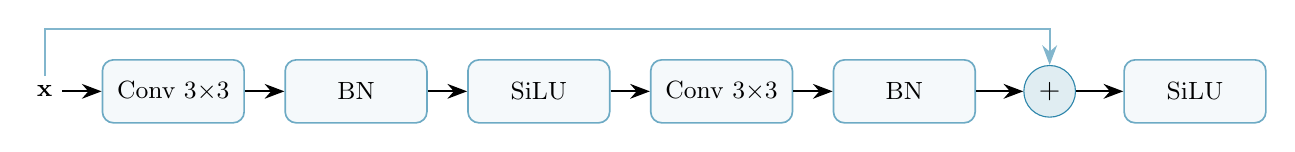
\begin{tikzpicture}[
    block/.style={rectangle, draw=vcolor!70, fill=vcolor!5, rounded corners, minimum height=0.8cm, minimum width=1.8cm, align=center, font=\small, line width=0.6pt},
    arr/.style={-{Stealth[length=2.5mm]}, thick},
  ]
    \node[block] (c1) {Conv 3$\times$3};
    \node[block, right=0.5cm of c1] (bn1) {BN};
    \node[block, right=0.5cm of bn1] (act1) {SiLU};
    \node[block, right=0.5cm of act1] (c2) {Conv 3$\times$3};
    \node[block, right=0.5cm of c2] (bn2) {BN};
    \node[circle, draw=vcolor, fill=vcolor!15, inner sep=3pt, font=\normalsize, right=0.6cm of bn2] (add) {$+$};
    \node[block, right=0.6cm of add] (act2) {SiLU};

    \draw[arr] (c1) -- (bn1);
    \draw[arr] (bn1) -- (act1);
    \draw[arr] (act1) -- (c2);
    \draw[arr] (c2) -- (bn2);
    \draw[arr] (bn2) -- (add);
    \draw[arr] (add) -- (act2);

    \node[left=0.5cm of c1, font=\small] (xin) {$\mathbf{x}$};
    \draw[arr] (xin) -- (c1);
    \draw[-{Stealth[length=2.5mm]}, vcolor!60, thick] (xin.north) -- ++(0,0.6) -| (add);
  \end{tikzpicture}%
  }
  \end{center}

  \vspace{0.3em}
  \small Channels: 32 $\to$ 64 $\to$ 128. Adding ResBlocks halved reconstruction error.
\end{frame}

\begin{frame}{FSQ-VAE: Training}
  \begin{itemize}
    \item $\sim$180K frames, batch 2048
    \item GRWM regularization (temporal slowness + uniformity)
    \item $\pm$4px random shift augmentation (edge padding)
    \item Cosine LR schedule, 200 epochs
    \item GPU: A100, total training time: $\sim$48 min
  \end{itemize}
\end{frame}

\begin{frame}{FSQ-VAE: Reconstructions}
  \begin{center}
    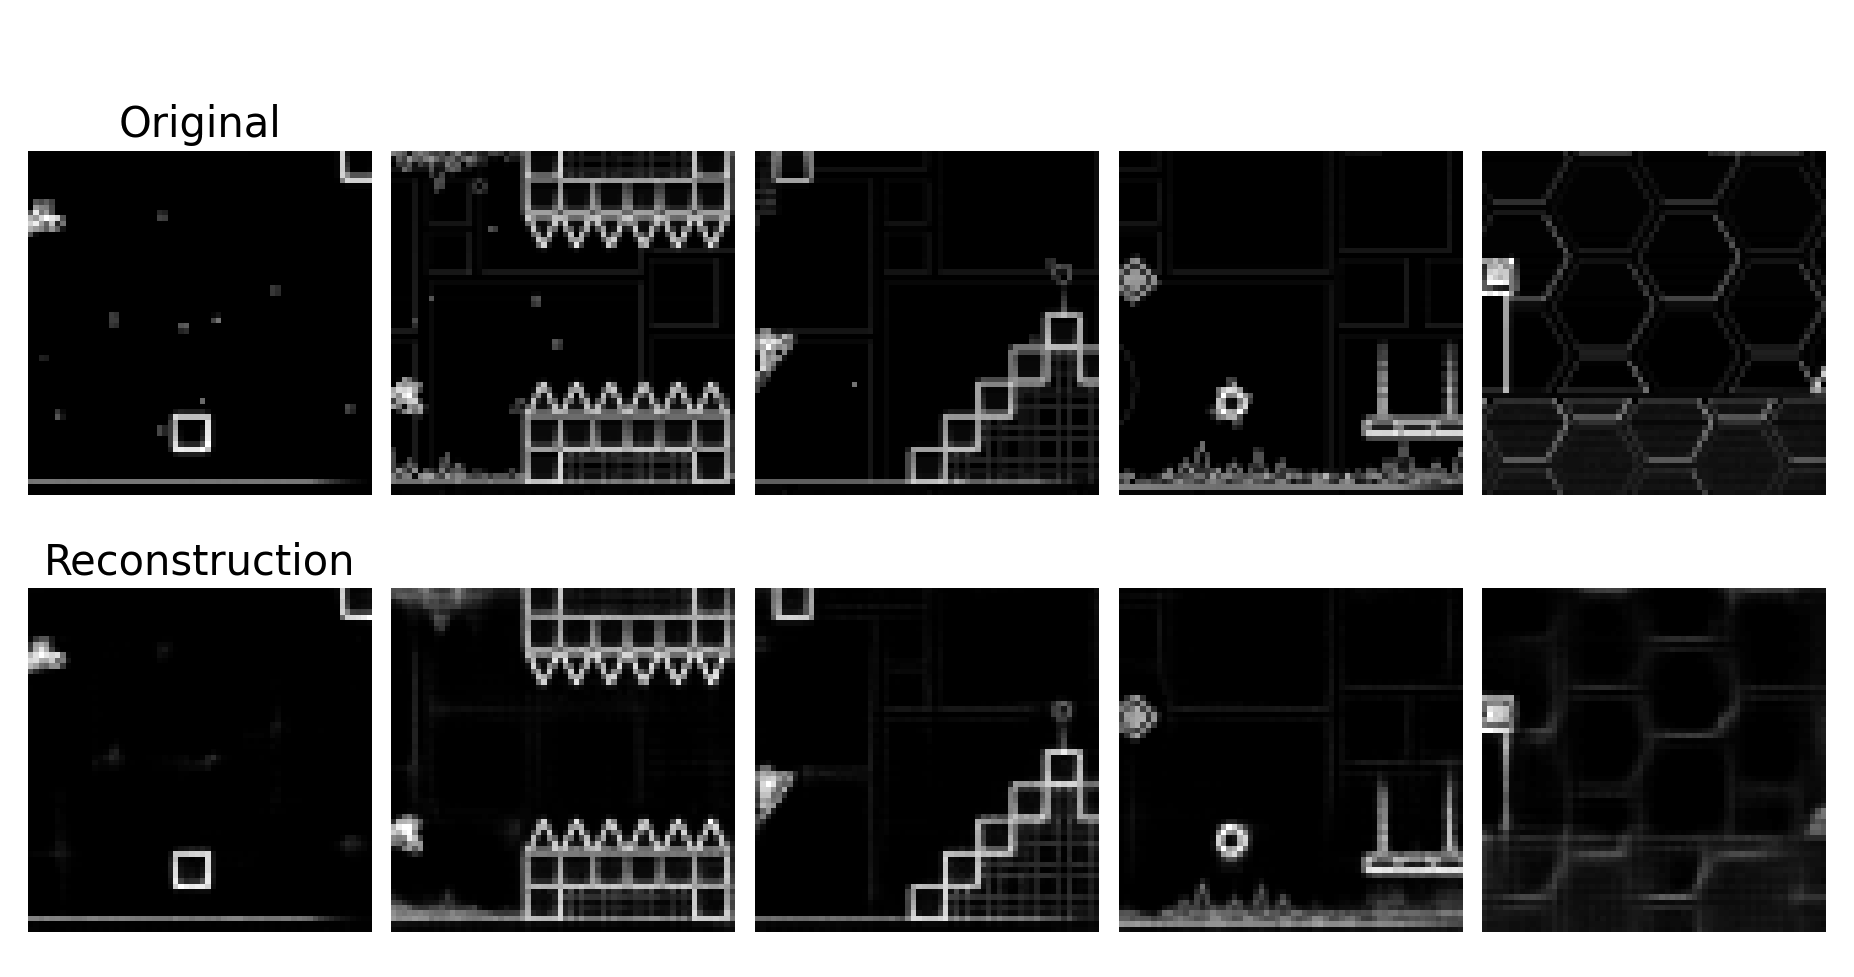
\includegraphics[width=\textwidth]{fsq_reconstructions.png}
  \end{center}
  \begin{center}
    \small RMSE $\approx 0.025$ per pixel
  \end{center}
\end{frame}

\begin{frame}{FSQ-VAE: Abstraction for Pipeline}
  \vspace{1em}
  \begin{center}
  \resizebox{\textwidth}{!}{%
  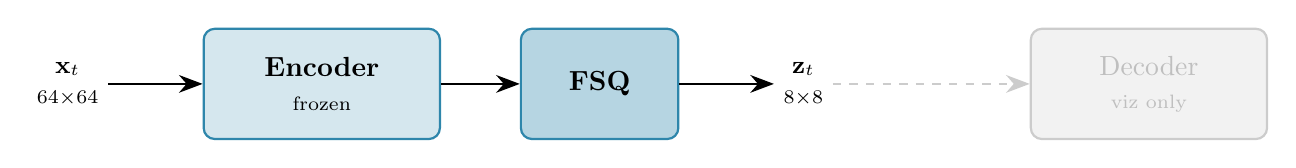
\begin{tikzpicture}[
    block/.style={rectangle, draw, rounded corners, minimum height=1.4cm, minimum width=3cm, align=center, font=\normalsize, line width=0.8pt},
    arr/.style={-{Stealth[length=3mm]}, thick},
    lbl/.style={font=\small, align=center},
  ]
    \node[lbl] (in) {$\mathbf{x}_t$\\{\scriptsize 64$\times$64}};
    \node[block, fill=vcolor!20, draw=vcolor, right=1.2cm of in] (enc) {\textbf{Encoder}\\{\scriptsize frozen}};
    \node[block, fill=vcolor!35, draw=vcolor, right=1cm of enc, minimum width=2cm] (fsq) {\textbf{FSQ}};
    \node[lbl, right=1.2cm of fsq] (out) {$\mathbf{z}_t$\\{\scriptsize 8$\times$8}};
    \node[block, fill=gray!10, draw=gray!40, right=2.5cm of out, text=gray!50] (dec) {Decoder\\{\scriptsize viz only}};

    \draw[arr] (in) -- (enc);
    \draw[arr] (enc) -- (fsq);
    \draw[arr] (fsq) -- (out);
    \draw[-{Stealth[length=3mm]}, gray!40, dashed, thick] (out) -- (dec);
  \end{tikzpicture}%
  }
  \end{center}

  \vspace{1em}
  \begin{itemize}
    \item Encoder + FSQ frozen after training, used in the full pipeline
    \item Decoder kept only for visualizing Transformer dream rollouts
    \item 51$\times$ compression: $64 \times 64 \times 8 = 32{,}768$ bits $\to$ $64 \times \underbrace{\lceil\log_2 1000\rceil}_{10} = 640$ bits
  \end{itemize}
\end{frame}

% ==========================================================
\section{Phase 2: M (Transformer)}
% ==========================================================

\begin{frame}{Transformer World Model: Architecture}
  \vspace{0.5em}
  \begin{center}
  \resizebox{\textwidth}{!}{%
  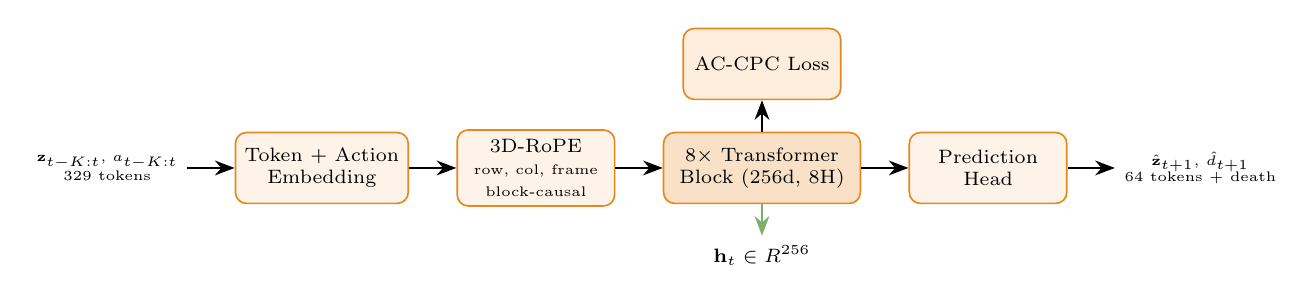
\begin{tikzpicture}[
    block/.style={rectangle, draw=mcolor, fill=mcolor!10, rounded corners, minimum height=0.9cm, align=center, font=\scriptsize, line width=0.6pt},
    arr/.style={-{Stealth[length=2.5mm]}, thick},
    lbl/.style={font=\tiny, align=center},
  ]
    \node[lbl] (in) {$\mathbf{z}_{t-K:t}$, $a_{t-K:t}$\\{\tiny 329 tokens}};
    \node[block, minimum width=2cm, right=0.6cm of in] (emb) {Token + Action\\Embedding};
    \node[block, minimum width=2cm, right=0.6cm of emb] (rope) {3D-RoPE\\{\tiny row, col, frame}\\{\tiny block-causal}};
    \node[block, minimum width=2.5cm, right=0.6cm of rope, fill=mcolor!25] (blocks) {8$\times$ Transformer\\Block (256d, 8H)};
    \node[block, minimum width=2cm, right=0.6cm of blocks] (head) {Prediction\\Head};
    \node[lbl, right=0.6cm of head] (out1) {$\hat{\mathbf{z}}_{t+1}$, $\hat{d}_{t+1}$\\{\tiny 64 tokens + death}};

    \node[block, minimum width=2cm, above=0.4cm of blocks, fill=mcolor!15] (cpc) {AC-CPC Loss};

    \draw[arr] (in) -- (emb);
    \draw[arr] (emb) -- (rope);
    \draw[arr] (rope) -- (blocks);
    \draw[arr] (blocks) -- (head);
    \draw[arr] (blocks) -- (cpc);
    \draw[arr] (head) -- (out1);

    \node[below=0.4cm of blocks, lbl, font=\scriptsize] (ht) {$\mathbf{h}_t \in \mathbb{R}^{256}$};
    \draw[arr, ccolor] (blocks.south) -- (ht);
  \end{tikzpicture}%
  }
  \end{center}

  \vspace{0.3em}
  \begin{center}
    \small
    6.7M params \quad\quad
    Parallel decode: 1 step vs 65 autoregressive \quad\quad
    Vocab: $|\mathcal{V}| = 1002$
  \end{center}
\end{frame}

\begin{frame}{Training: Spatial Shift Augmentation}
  \textbf{Problem}: 3,600 episodes is limited data for 6.7M params $\Rightarrow$ overfitting

  \vspace{0.3em}
  \textbf{Solution}: re-encode frames through frozen FSQ-VAE at pixel offsets

  \begin{center}
  \resizebox{0.85\textwidth}{!}{%
  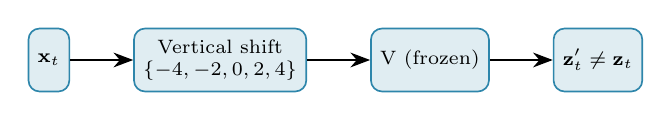
\begin{tikzpicture}[
    block/.style={rectangle, draw=vcolor, fill=vcolor!15, rounded corners, minimum height=0.8cm, align=center, font=\scriptsize, line width=0.6pt},
    arr/.style={-{Stealth[length=2.5mm]}, thick},
    lbl/.style={font=\tiny, align=center},
  ]
    \node[block] (frame) {$\mathbf{x}_t$};
    \node[block, right=0.8cm of frame] (shift) {Vertical shift\\$\{-4,-2,0,2,4\}$};
    \node[block, right=0.8cm of shift] (enc) {V (frozen)};
    \node[block, right=0.8cm of enc] (tok) {$\mathbf{z}'_t \neq \mathbf{z}_t$};

    \draw[arr] (frame) -- (shift);
    \draw[arr] (shift) -- (enc);
    \draw[arr] (enc) -- (tok);
  \end{tikzpicture}%
  }
  \end{center}

  \begin{itemize}
    \item 5 vertical shifts $\times$ 3,582 episodes $=$ \textbf{17,910 augmented episodes}
    \item Vertical shifts simulate different jump heights (physically valid)
    \item Horizontal shifts removed: player X position is fixed in Geometry Dash
    \item Edge padding (same as FSQ-VAE training)
  \end{itemize}
\end{frame}

\begin{frame}{Training: Dual Token Noise}
  \vspace{0.5em}
  \begin{columns}[T]
    \column{0.55\textwidth}
    Two complementary noise types on context tokens:

    \vspace{0.5em}
    \textbf{1. Random replacement (5\%)}
    \begin{itemize}
      \item Any of 1000 tokens uniformly
      \item Forces global robustness
    \end{itemize}

    \vspace{0.5em}
    \textbf{2. FSQ neighbor substitution (5\%)} {\color{insared}\textit{(novel)}}
    \begin{itemize}
      \item $\pm1$ in one FSQ dimension
      \item Visually near-identical patches
      \item Forces embedding to learn codebook topology
    \end{itemize}

    \column{0.45\textwidth}
    \vspace{-1.2em}
    \begin{center}
      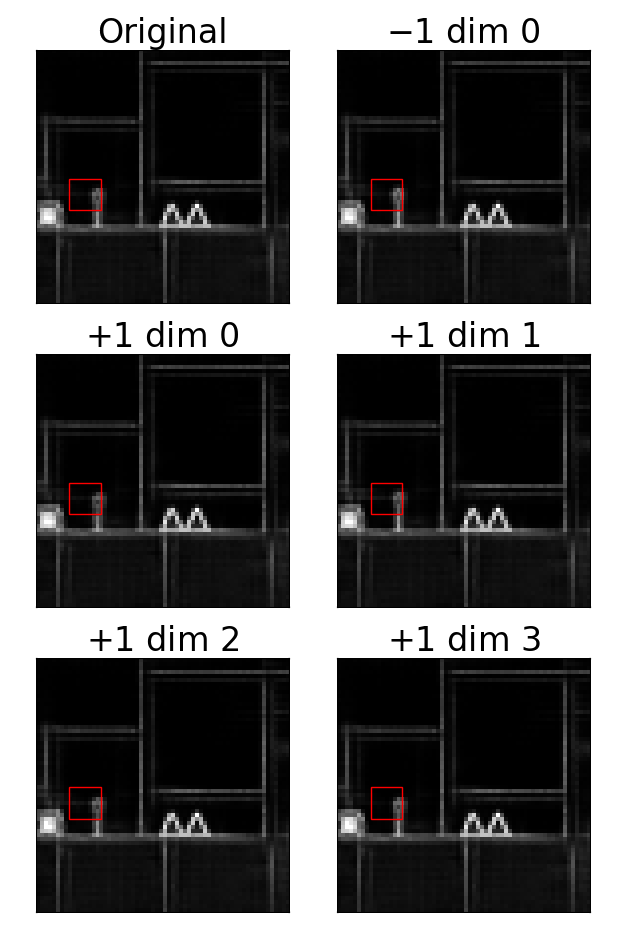
\includegraphics[width=0.80\textwidth]{fsq_neighbors.png}
    \end{center}
  \end{columns}
\end{frame}

\begin{frame}[t]{Novel: FSQ-Structured Label Smoothing}
  \textbf{Problem}: standard label smoothing spreads probability \emph{uniformly}. A $\pm1$ neighbor (visually identical) gets the same target mass as a completely unrelated token.

  \vspace{0.5em}
  \textbf{Solution} {\color{insared}\textit{(novel)}}: Gaussian kernel over squared FSQ coordinate distance:
  \[
    w(a,b) = \exp\!\left(-\frac{d^2(a,b)}{2\sigma^2}\right), \quad d^2 = \sum_i (\Delta_i)^2, \quad \sigma = 0.9
  \]

  $\sigma$ calibrated from empirical MSE analysis (800 samples per perturbation):

  \vspace{0.2em}
  \begin{center}
    \small
    \begin{tabular}{lcc}
      \toprule
      Perturbation & Patch MSE & Ratio \\
      \midrule
      $\pm1$ single dim & 0.000078 & 1.0$\times$ \\
      $+1$ two dims & 0.000200 & 2.55$\times$ \\
      $+2$ single dim & 0.000493 & \textbf{6.30$\times$} \\
      \bottomrule
    \end{tabular}
  \end{center}

  \vspace{0.2em}\end{frame}

\begin{frame}{Dream Rollout}
  \vspace{0.5em}
  \begin{center}
  \resizebox{0.85\textwidth}{!}{%
  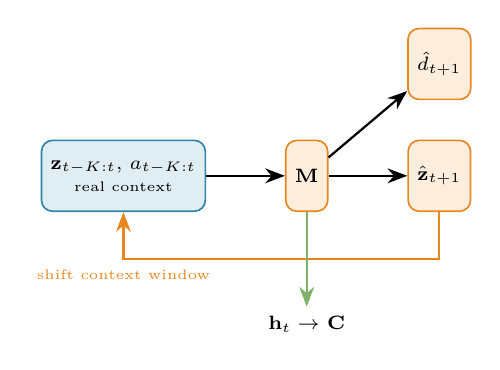
\begin{tikzpicture}[
    block/.style={rectangle, draw=mcolor, fill=mcolor!15, rounded corners, minimum height=0.9cm, align=center, font=\scriptsize, line width=0.6pt},
    arr/.style={-{Stealth[length=2.5mm]}, thick},
    lbl/.style={font=\tiny, align=center},
  ]
    \node[block, fill=vcolor!15, draw=vcolor] (ctx) {$\mathbf{z}_{t-K:t}$, $a_{t-K:t}$\\{\tiny real context}};
    \node[block, right=1cm of ctx] (tfm) {\textbf{M}};
    \node[block, right=1cm of tfm] (pred) {$\hat{\mathbf{z}}_{t+1}$};
    \node[block, above=0.5cm of pred] (death) {$\hat{d}_{t+1}$};

    \draw[arr] (ctx) -- (tfm);
    \draw[arr] (tfm) -- (pred);
    \draw[arr] (tfm) -- (death);

    \draw[arr, mcolor] (pred.south) -- ++(0,-0.6) -| node[below, lbl, pos=0.5] {shift context window} (ctx.south);

    \node[below=1.2cm of tfm, font=\scriptsize] (ht) {$\mathbf{h}_t \to$ \textbf{C}};
    \draw[arr, ccolor] (tfm.south) -- ++(0,-0.3) -- (ht);
  \end{tikzpicture}%
  }
  \end{center}

  \vspace{0.5em}
  \begin{itemize}
    \item Warmup: $K=4$ real frames as ground truth context
    \item Dream: autoregressive prediction using own outputs
    \item $\mathbf{h}_t$ feeds the controller; rollout stops when $\hat{d}_{t+1} > 0.5$
  \end{itemize}
\end{frame}

\begin{frame}{Transformer: Training Results}
  \textbf{V1 Final} (200 epochs, LR $2 \times 10^{-3}$, 5$\times$ death oversample, vertical-only shifts):

  \vspace{0.5em}
  \begin{center}
    \small
    \begin{tabular}{lccc}
      \toprule
      Metric & Baseline & Overfitted (400ep) & \textbf{V1 Final} \\
      \midrule
      Val accuracy & 33.66\% & 34.69\% & \textbf{36.06\%} \\
      Val token loss & 2.383 & 2.327 & \textbf{2.255} \\
      Death precision & -- & 48.4\% & \textbf{61.0\%} \\
      Death F1 & -- & 63.5\% & \textbf{71.7\%} \\
      Death P gap (train-val) & -- & 44pp & \textbf{28pp} \\
      \bottomrule
    \end{tabular}
  \end{center}

  \vspace{0.5em}
  \begin{itemize}
    \item Key fix: death oversample $15\times \to 5\times$ (eliminated death pattern memorization)
    \item Expert episodes (33K frames) teach model that obstacles are survivable
  \end{itemize}
\end{frame}

% ==========================================================
\section{Phase 3: C (Controller)}
% ==========================================================

\begin{frame}{Controller: Architecture}
  \textbf{CNNPolicy} (40K params): CNN actor-critic on 8$\times$8 token grid

  \vspace{0.5em}
  \begin{center}
  \resizebox{0.9\textwidth}{!}{%
  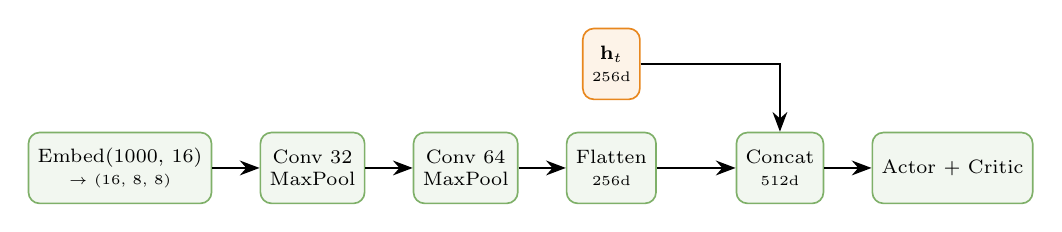
\begin{tikzpicture}[
    block/.style={rectangle, draw=ccolor, fill=ccolor!10, rounded corners, minimum height=0.9cm, align=center, font=\scriptsize, line width=0.6pt},
    arr/.style={-{Stealth[length=2.5mm]}, thick},
    lbl/.style={font=\tiny, align=center},
  ]
    \node[block] (emb) {Embed(1000, 16)\\{\tiny $\to$ (16, 8, 8)}};
    \node[block, right=0.6cm of emb] (c1) {Conv 32\\MaxPool};
    \node[block, right=0.6cm of c1] (c2) {Conv 64\\MaxPool};
    \node[block, right=0.6cm of c2] (flat) {Flatten\\{\tiny 256d}};
    \node[block, fill=mcolor!10, draw=mcolor, above=0.4cm of flat] (ht) {$\mathbf{h}_t$\\{\tiny 256d}};
    \node[block, right=1cm of flat] (cat) {Concat\\{\tiny 512d}};
    \node[block, right=0.6cm of cat] (heads) {Actor + Critic};

    \draw[arr] (emb) -- (c1);
    \draw[arr] (c1) -- (c2);
    \draw[arr] (c2) -- (flat);
    \draw[arr] (flat) -- (cat);
    \draw[arr] (ht) -| (cat);
    \draw[arr] (cat) -- (heads);
  \end{tikzpicture}%
  }
  \end{center}

  \vspace{0.5em}
  Inputs: token grid $\mathbf{z}_t \in \{0,\ldots,999\}^{64}$ + hidden state $\mathbf{h}_t \in \mathbb{R}^{256}$
\end{frame}

\begin{frame}{Controller: Training Protocol}
  \textbf{Stage 1: Behavioral Cloning} (initialization)
  \begin{itemize}
    \item Death + expert episodes, class-weighted BCE (2.6$\times$ jump weight)
    \item Feed context through world model $\to$ get $\mathbf{h}_t$, predict expert action
    \item Val accuracy: 78\% (above 72\% always-idle baseline)
  \end{itemize}

  \vspace{0.5em}
  \textbf{Stage 2: PPO in Dream} (generalization)
  \begin{itemize}
    \item Uniform context sampling, excluding last $2K$ frames per episode
    \item Reward: $+1$ per step survived, rollout stops at death prediction
    \item 512 episodes/iteration, 4 PPO epochs, GAE ($\gamma$=0.995, $\lambda$=0.95)
    \item 9K iterations: eval survival $19.86 \to 23.04$
  \end{itemize}

  \vspace{0.5em}
  \textbf{Test:} zero-shot deployment on \emph{unseen} levels
\end{frame}

% ==========================================================
\section{Full Inference Pipeline}
% ==========================================================

\begin{frame}{Inference: Assembling the Pipeline}
  At inference, the prediction head is pruned. Only $\mathbf{h}_t$ matters.

  \vspace{0.5em}
  \begin{center}
  \resizebox{\textwidth}{!}{%
  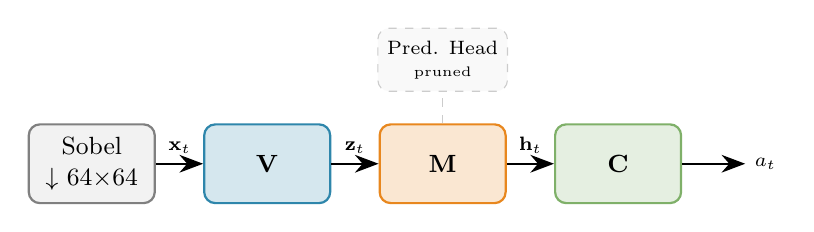
\begin{tikzpicture}[
    block/.style={rectangle, draw, rounded corners, minimum height=1cm, align=center, font=\small, line width=0.8pt},
    arr/.style={-{Stealth[length=3mm]}, thick},
    lbl/.style={font=\scriptsize, align=center},
    ghost/.style={rectangle, draw=gray!40, fill=gray!5, rounded corners, minimum height=0.8cm, align=center, font=\scriptsize, dashed},
  ]
    \node[block, fill=gray!10, draw=gray, minimum width=1.6cm] (pre) {Sobel\\$\downarrow$ 64$\times$64};
    \node[block, fill=vcolor!20, draw=vcolor, right=0.6cm of pre, minimum width=1.6cm] (enc) {\textbf{V}};
    \node[block, fill=mcolor!20, draw=mcolor, right=0.6cm of enc, minimum width=1.6cm] (tfm) {\textbf{M}};
    \node[block, fill=ccolor!20, draw=ccolor, right=0.6cm of tfm, minimum width=1.6cm] (ctrl) {\textbf{C}};
    \node[lbl, right=0.8cm of ctrl] (act) {$a_t$};

    \node[ghost, above=0.4cm of tfm] (pred) {Pred. Head\\{\tiny pruned}};
    \draw[gray!40, dashed] (tfm) -- (pred);

    \draw[arr] (pre) -- node[above, lbl] {$\mathbf{x}_t$} (enc);
    \draw[arr] (enc) -- node[above, lbl] {$\mathbf{z}_t$} (tfm);
    \draw[arr] (tfm) -- node[above, lbl] {$\mathbf{h}_t$} (ctrl);
    \draw[arr] (ctrl) -- (act);
  \end{tikzpicture}%
  }
  \end{center}

  \vspace{0.5em}
  \begin{center}
    \small
    Screen capture at 30 FPS $\to$ Sobel $\to$ V $\to$ M $\to$ C $\to$ game input \\[0.3em]
    Game stepped every 8 ticks at 240 TPS $=$ 30 decisions/sec
  \end{center}
\end{frame}

\begin{frame}{Deployment: Real-Time at 30 FPS}
  \begin{center}
    \small
    \begin{tabular}{lcc}
      \toprule
      Stage & Time (ms) & \% Budget \\
      \midrule
      Screen capture & 2.5 & 9\% \\
      Sobel preprocessing & 9.0 & 33\% \\
      FSQ encoding & 4.5 & 16\% \\
      Transformer ($\mathbf{h}_t$) & 9.0 & 33\% \\
      Controller & 1.5 & 5\% \\
      \midrule
      \textbf{Total} & \textbf{26.5} & -- \\
      \textbf{Budget (30 FPS)} & \textbf{33.3} & -- \\
      \bottomrule
    \end{tabular}
  \end{center}

  \vspace{0.5em}
  \begin{itemize}
    \item First known real-time World Models deployment
    \item Agent dodges simple obstacles (single/double spikes)
    \item Struggles with complex obstacle sequences (jumps too early/often)
  \end{itemize}
\end{frame}

% ==========================================================
\section{Analysis}
% ==========================================================

\begin{frame}{What Worked}
  \begin{itemize}
    \item \textbf{FSQ-VAE}: sharp reconstructions, 100\% codebook utilization, no tuning headaches
    \item \textbf{Sobel preprocessing}: filters visual noise, forces structural perception
    \item \textbf{Vertical shift augmentation}: reduced overfitting, physically valid for side-scrollers
    \item \textbf{Parallel decoding}: all 65 tokens in 1 forward pass vs 65 autoregressive. Critical for real-time play
    \item \textbf{Structured label smoothing}: empirically grounded via FSQ distance analysis
  \end{itemize}
\end{frame}

\begin{frame}{What Didn't Work (or Didn't Help)}
  \begin{itemize}
    \item \textbf{$\beta$-VAE}: fundamentally blurry. Wide range of hyperparameter search before switching to VQ/FSQ
    \item \textbf{LR $10^{-3}$ without augmentation}: 13.5pp train/val gap at epoch 29, model memorizing
    \item \textbf{FSQ neighbor substitution}: no measurable accuracy impact (same curves), but theoretically sound and free to keep
    \item \textbf{Pure RL controller}: CMA-ES, REINFORCE, PPO all flatlined at $\sim$12 steps. BC pretraining required
    \item \textbf{Death-only training data}: 15$\times$ death oversample caused memorization (44pp precision gap). Fixed: 5$\times$ + expert episodes
    \item \textbf{MaskGIT iterative decoding}: degraded dream quality on 64-token grid. Parallel single-step works better (bidirectional attention sufficient)
    \item \textbf{torch.compile on full model}: 23+ min compilation. Solved by compiling backbone only
  \end{itemize}
\end{frame}

% ==========================================================
\section{Limitations}
% ==========================================================

\begin{frame}{Limitations \& Future Work}
  \begin{itemize}
    \item \textbf{Controller precision}: jumps too often/early, struggles with complex obstacle sequences
    \item \textbf{Dream/reality gap}: controller trained in imagination, h$_t$ distribution may differ in real game
    \item \textbf{Sobel bottleneck}: CPU Sobel on 1032$\times$1032 takes 9ms (33\% of frame budget). GPU Sobel requires FSQ retraining
    \item \textbf{AC-CPC underutilized}: weight 0.1 (TWISTER uses 1.0), 1-step horizon (TWISTER uses 10). h$_t$ may not encode enough temporal context
    \item \textbf{Token-level augmentation}: can't crop/resize once tokenized (tokens are patch-specific)
  \end{itemize}
\end{frame}

% ==========================================================
\section{References}
% ==========================================================

\begin{frame}[allowframebreaks]{References}
  \small
  \begin{itemize}
    \item Micheli, V. et al. (2023). \textit{Transformers are Sample-Efficient World Models} (IRIS). arXiv:2209.00588
    \item Ha, D. \& Schmidhuber, J. (2018). \textit{World Models}. arXiv:1803.10122
    \item Mentzer, F. et al. (2023). \textit{Finite Scalar Quantization: VQ-VAE Made Simple}. arXiv:2309.15505
    \item Burchert, J. et al. (2025). \textit{TWISTER: Learning Transformer-based World Models with AC-CPC}. arXiv:2503.04416
    \item Hafner, D. et al. (2023). \textit{Mastering Diverse Domains through World Models} (DreamerV3). arXiv:2301.04104
    \item Schulman, J. et al. (2017). \textit{Proximal Policy Optimization Algorithms}. arXiv:1707.06347
    \item Szegedy, C. et al. (2016). \textit{Rethinking the Inception Architecture for Computer Vision}. (Label smoothing)
    \item Lin, T.-Y. et al. (2017). \textit{Focal Loss for Dense Object Detection}. ICCV
  \end{itemize}
\end{frame}

\end{document}
